\chapter{Конструкторский раздел}
\label{cha:design}

\section{Выполняемые задачи}

Основная задача данной работы - удаление подписей из текстов электронных писем.

На рисунке \ref{design:idef_0} показана диаграмма IDEF0, которая отображает основные этапы удаления подписей из текстов электронных писем.

\begin{figure}[h!]
	\centering
	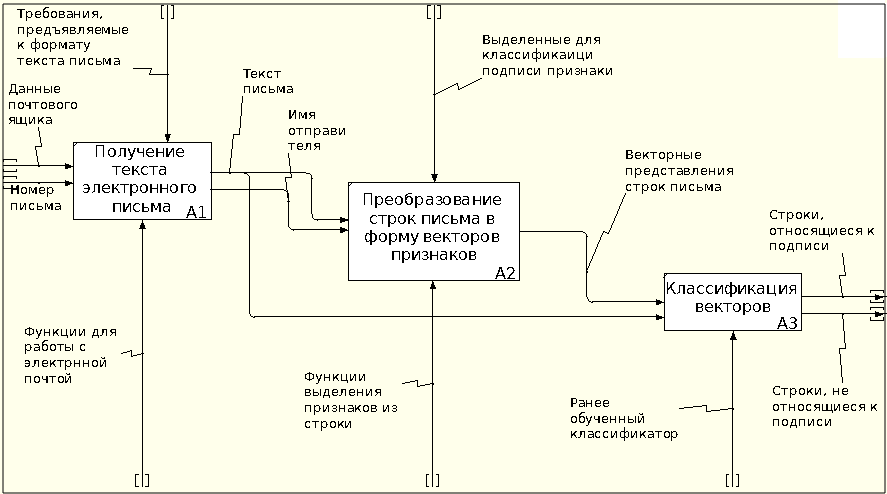
\includegraphics[width=\textwidth]{inc/img/idef_0.png}
	\caption{IDEF0-диаграмма проекта}
	\label{design:idef_0}
\end{figure}

Как видно из рисунка, данную задачу можно разделить на три основных этапа:

\begin{itemize}
	\item получение текста электронного письма;
	\item преобразование строк письма в форму векторов признаков;
	\item классификация векторов, полученных на предыдущем этапе.
\end{itemize}

\newpage
\section{Получение текста электронного письма}
На данном этапе решается задача получения текста электронного письма из почтового ящика пользователя. Соответственно, входными данными будут являться данные электронного почтового ящика(адрес, пароль), а также номер того письма, текст которого необходимо получить. В результате, помимо текста письма, будет получено еще и значение заголовка "From", оно будет использовано в следующем этапе для приведения строк письма к формату вектора признаков. 

Так как в настоящее время, в теле письма может передаваться практически любая по типу информация, то введем ограничение, согласно которому тексту письма будет соответствовать только информация, имеющая значение "text/plain" заголовка "Content-type". Выделение текста из элементов типа "text/html" выходит за рамки разрабатываемого метода и может быть рассмотрено как расширение функционала разрабатываемого программного обеспечения.

На рисунке \ref{design:alg-email} представлена схема работы алгоритма получения текста электронного письма.

\newpage
\begin{figure}[h!]
	\centering
	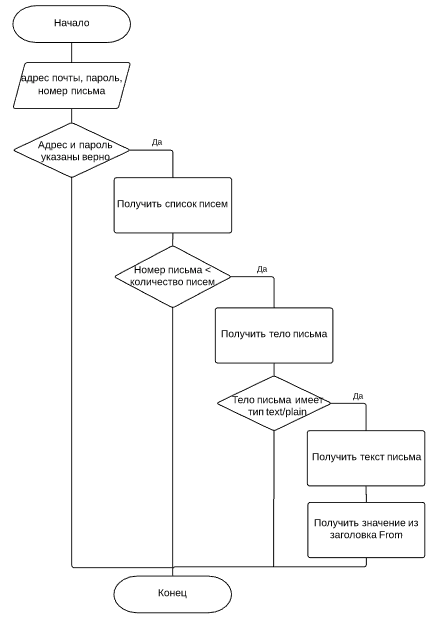
\includegraphics[width=\textwidth]{inc/img/alg-email.png}
	\caption{Схема алгоритма получения электронного письма}
	\label{design:alg-email}
\end{figure}

\section{Преобразование строк письма в форму векторов признаков}
Для решения задачи классификации необходимо представить классифицируемые объекты, в данном случае строки текста электронного письма, в форме числовых векторов. В аналитическом разделе были описаны основные подходы, применяемые для приведения классифицируемых объектов к необходимому виду. В рамках текущей работы выбор был сделан в пользу метода, основанного на представлении строки в виде вектора признаков.
С целью определения строк, относящихся к подписи, были выделены, следующие признаки:

\begin{itemize}
	\item строка содержит адрес электронной почты;
	\item строка содержит URL адрес;
	\item строка представлена в виде разделителя типа "------";
	\item строка содержит номер телефона;
	\item строка содержит имя человека;
	\item строка содержит часто употребимые слова (Спасибо, с уважением и т.п.);
	\item процент слов, начинающихся с заглавной буквы, в строке не менее 50; 
	\item процент цифр среди общего количества всех символов в строке не менее 30;
	\item длина строки не более 50 символов;
	\item строка содержит имя отправителя, полученное из заголовка "From" электронного письма;
\end{itemize}

В результате выделения описанных выше признаков, строка текста электронного письма будет представлена в виде вектора $v$ = ($v_1$,$v_2$...,$v_n$), где $n$ - количество выделенных признаков. Элементы вектора $v$ могут принимать два значения: 0 и 1, где 0 - данный признак отсутствует в строке, 1 - присутствует. 

Например, для строки <С уважением, Мельников Дмитрий>, полученной из письма, отправленного от имени <Мельников Д. citrus\_m@mail.ru>, cоответствующий вектор будет выглядеть следующим образом: (0, 0, 0, 0, 1, 1, 1, 0, 1, 1).

Стоит заметить, что первые 6 шесть описанных признаков могут быть выделены из строки с использованием регулярных выражений.
Данные регулярные выражения представлены в приложении А.

На рисунке \ref{design:alg-features} представлена схема алгоритма преобразования строк письма в вектора признаков.

\begin{figure}[h!]
	\centering
	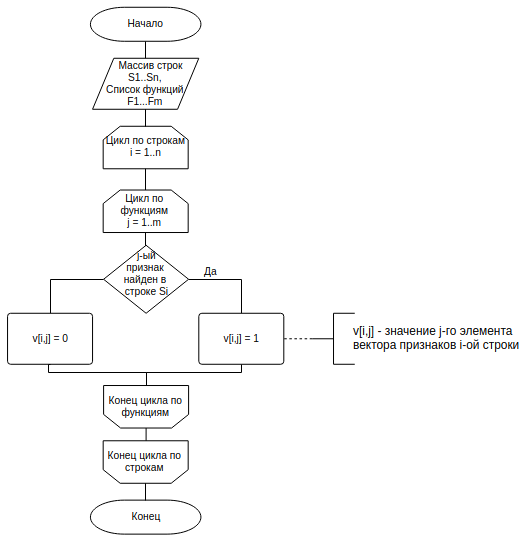
\includegraphics[width=\textwidth]{inc/img/alg-features.png}
	\caption{Схема алгоритма преобразования строк письма в вектора признаков}
	\label{design:alg-features}
\end{figure}


\section{Классификация векторов признаков}
Последним этапом выделения подписи является классификация числовых векторов, описывающих строки письма. Для решения данной задачи необходимо иметь заранее обученный классификатор.
Поэтому следует описать набор действий, необходимых для получения обученной модели классификатора.

\subsection{Описание обучающей выборки данных}
Так как для решения задач классификации используются алгоритмы обучения с учителем, то возникает необходимость разметки обучающей выборки с целью указания метки класса, к которому принадлежит классифицируемый объект.

В данной работе исходные данные представляют из себя множество из пар файлов, в которых один файл содержит текст электронного письма, а другой - значение, полученное из заголовка From, которое используется для выделения последнего из ранее описанных признаков. Разметке подлежит файл, содержащий текст письма. Пример размеченного файла представлен на рисунке \ref{design:email-dataset}.


\begin{figure}[h!]
	\centering
	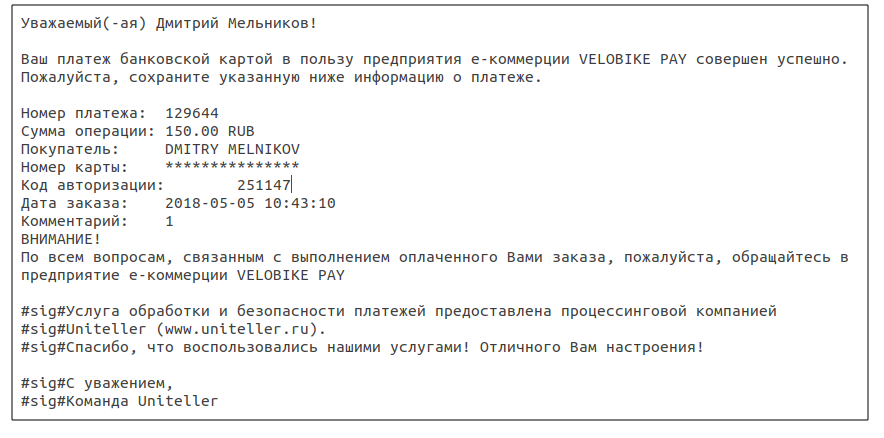
\includegraphics[width=\textwidth]{inc/img/email_dataset.png}
	\caption{Пример разметки текста электронного письма}
	\label{design:email-dataset}
\end{figure}

Префикс \#sig\# означает, что строка относится к классу "подпись". 

\subsection{Обучение классификатора}
На рисунке \ref{design:idef_1} представлена IDEF0 диаграмма, описывающая основные этапы получения обученной модели классификатора.

Как видно из рисунка, данную задачу можно разделить на 4 основных этапа:

\begin{itemize}
	\item Разметка текстов электронных писем;
	\item Приведение строк электронных писем к виду векторов признаков;
	\item Добавления данных для обучения в БД;
	\item Обучение классификатора;
\end{itemize}

\begin{figure}[h!]
	\centering
	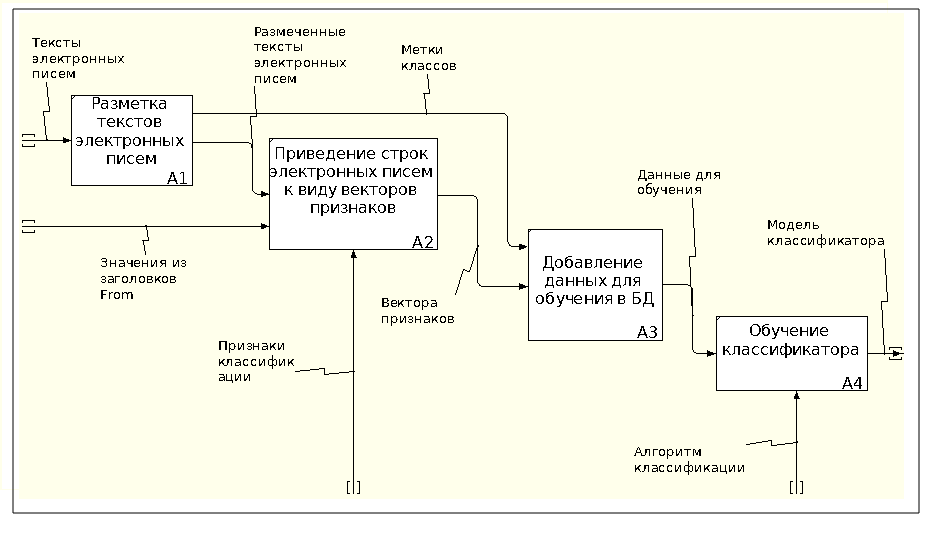
\includegraphics[width=\textwidth]{inc/img/idef_1.png}
	\caption{IDEF-диаграмма получения обученной модели классификатора}
	\label{design:idef_1}
\end{figure}

Стоит обратить внимание на то, что третий этап не является обязательным, однако, использование базы данных для хранения обучающей выборки позволяет удобно расширять выборку за счет добавления новых писем, а также позволяет быстрее производить обучение классификатора.

\section{Структура программы}

Общая структура разработанного программного комплекса представлена на рисунке \ref{design:modules}

\begin{figure}[h!]
	\centering
	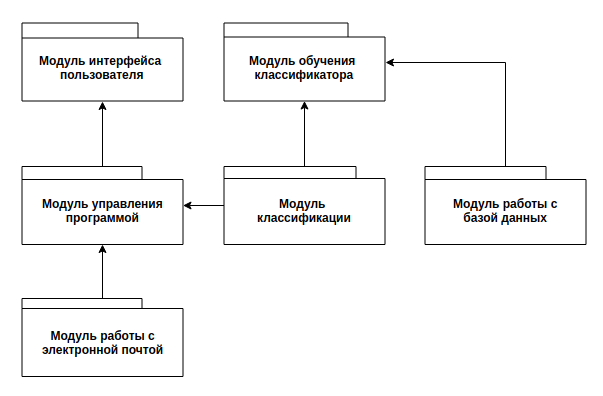
\includegraphics[width=\textwidth]{inc/img/modules.png}
	\caption{Структура программного комплекса}
	\label{design:modules}
\end{figure}

Разработанный программный комплекс можно разделить на две части: пользовательское приложение с графическим интерфейсом и приложение для получения обученной модели классификатора. 
Основой пользовательского приложения является модуль управления программой, который содержит в себе основную логику работы приложения и осуществляет взаимодействие других компонентов приложения: модулей классификации, работы с электронной почтой и интерфейса пользователя.

Функционал, используемый обеими частями программного комплекса, представлен только в модуле классификации, при этом для работы пользовательского приложения не требуется наличия модуля работы с базой данных.

\section{Выводы}
В конструкторском разделе описывается предлагаемый метод удаления подписей из текстов электронных писем. Дано подробное описание, построены схемы выбранных алгоритмов. При этом выделены основные этапы работы метода с указанием необходимых исходных данных для его работы и полученных результатов на каждом этапе.
%%% Local Variables:
%%% mode: latex
%%% TeX-master: "rpz"
%%% End:
